\documentclass[../structural_economics_book.tex]{subfiles}
\begin{document}
\ifSubfilesClassLoaded{\setcounter{chapter}{19}}{}
\chapter{Social Accounting Matrices as Weight Matrices}\label{ch:20}
\chaptersubtitle{The Data Infrastructure of Structural Economics}
\begin{quote}
\textit{``A structuralist model of the economy rests on three pillars: a social accounting matrix to describe the flows, a set of closure rules to determine which variables adjust, and a theory of distribution to explain who gets what.''}\\
\hfill --- Lance Taylor, \textit{Structuralist Macroeconomics} (1983)
\end{quote}

\vspace{1em}

Parts~I--V developed the theory. Part~VI builds the measurement infrastructure. The question is no longer ``what does $W$ imply?'' but ``where does $W$ come from?''

The answer, for the production network $W^P$, is the Social Accounting Matrix (SAM): a square matrix that records every flow between every pair of accounts in the economy. The SAM IS the weight matrix --- or rather, the row-normalized SAM is $W^P$. Every proposition, theorem, and diagnostic from the previous 19 chapters can be computed from a SAM.

This chapter shows how. It translates the entire framework into SAM language, constructs Bolivia's SAM, and runs the structural diagnostics from Chapter~17 on actual data. The remaining chapters in Part~VI extend the measurement to $W^I$ (Chapter~21), $W^U$ (Chapter~22), and time series (Chapter~23).


%% =====================================================================
\section{The SAM as the Complete Flow Matrix}
\label{ch20:sec:sam}
%% =====================================================================

\subsection{Definition}

\begin{definition}[Social Accounting Matrix]\label{ch20:def:sam}
A \textbf{Social Accounting Matrix} is an $M \times M$ matrix $T$ where:
\begin{enumerate}
\item Each row and column represents an \textbf{account}: a production sector, a factor of production (labor, capital), a household group, a government account, a capital account, or the rest of the world.
\item Entry $T_{ij}$ records the total payment from account $j$ (column) to account $i$ (row) during the accounting period.
\item Row sums equal column sums for every account: $\sum_j T_{ij} = \sum_j T_{ji}$ for all $i$. The SAM is balanced by construction (every dollar paid by one account is received by another).
\end{enumerate}
\end{definition}

The SAM generalizes the I-O table in two directions: it includes factors and institutions (not just production sectors), and it records the \textit{complete} circular flow of income --- from production to factors to households to consumption to production.

\begin{definition}[SAM Accounts --- Standard Classification]\label{ch20:def:accounts}
\begin{center}
\begin{tabular}{lll}
\toprule
\textbf{Account type} & \textbf{Examples} & \textbf{Role in $W$} \\
\midrule
Production activities & Agriculture, Manufacturing, Gas & $W^P$ entries \\
Commodities & Goods and services (supply/demand) & Market clearing \\
Factors & Labor (by type), Capital & Factor payments \\
Households & By income quintile, urban/rural, ethnicity & $W^U$ entries \\
Government & Tax, transfers, public spending & Policy instruments \\
Capital account & Savings, investment & Accumulation \\
Rest of world & Exports, imports, remittances & Global linkage \\
\bottomrule
\end{tabular}
\end{center}
\end{definition}

\subsection{From the SAM to $W^P$}

\begin{definition}[The SAM-Derived Weight Matrix]\label{ch20:def:sam_to_W}
Row-normalize the SAM to obtain the weight matrix:
\begin{equation}\label{ch20:eq:sam_to_W}
W_{ij} = \frac{T_{ij}}{\sum_k T_{ik}}.
\end{equation}
Entry $W_{ij}$ is the share of account $i$'s total receipts that comes from account $j$. This is a row-stochastic matrix. The Perron eigenvector, spectral gap, and all derived quantities are computable directly from $W$.
\end{definition}

\begin{proposition}[The SAM Contains $W^P$ as a Submatrix]\label{ch20:prop:submatrix}
The production-activities block of the SAM (rows and columns corresponding to production sectors) yields the I-O matrix $A$ (Chapter~1). Row-normalizing $A$ gives $W^P$. The full SAM-derived $W$ extends $W^P$ by including factor payments, household income, and government transfers --- capturing all the channels through which economic power flows.

The full SAM-derived $W$ is \textit{larger} and \textit{richer} than $W^P$ alone:
\begin{enumerate}
\item $W^P$ captures inter-sectoral production linkages only.
\item The full $W$ also captures factor-payment linkages (which sectors pay which factors), distributional linkages (which factors go to which households), and fiscal linkages (government taxation and transfers).
\item The spectral gap of the full $W$ is generally \textit{smaller} than $\Gamma(W^P)$ because the additional accounts introduce new blocks (factor types, household groups) with weak cross-block links.
\end{enumerate}
\end{proposition}


%% =====================================================================
\section{Constructing Bolivia's SAM}
\label{ch20:sec:bolivia_sam}
%% =====================================================================

\subsection{Data Sources}

\begin{example}[Bolivia SAM, 2016 --- Data Assembly]\label{ch20:ex:data}
\begin{center}
\begin{tabular}{lll}
\toprule
\textbf{SAM block} & \textbf{Data source} & \textbf{Detail} \\
\midrule
Production $\times$ Production & INE I-O table 2016 & 35 sectors \\
Production $\times$ Factors & National Accounts & Value added by sector \\
Factors $\times$ Households & EH 2016 & Wages, profits by HH type \\
Households $\times$ Commodities & EH 2016 (consumption) & Expenditure by HH type \\
Government $\times$ all & Fiscal data (MEFP) & Tax, transfers, spending \\
Rest of world & Balance of payments & Exports, imports, FDI \\
\bottomrule
\end{tabular}
\end{center}
\end{example}

\subsection{The SAM Structure}

\begin{example}[Bolivia SAM, 2016 --- Aggregated to $10 \times 10$]\label{ch20:ex:bolivia_sam}
Aggregate to 10 accounts: (1) Gas/Mining, (2) Agriculture, (3) Manufacturing, (4) Services, (5) Labor, (6) Capital, (7) Poor Households, (8) Non-Poor Households, (9) Government, (10) Rest of World.

\begin{center}
\small
\begin{tabular}{l|rrrrrrrrrr}
\toprule
& Gas & Agr & Mfg & Svc & Lab & Cap & HH-P & HH-NP & Gov & RoW \\
\midrule
Gas & 2.1 & 0.1 & 0.8 & 0.3 & & & & & 0.2 & 4.5 \\
Agr & 0.0 & 1.8 & 1.5 & 0.5 & & & & & 0.1 & 0.8 \\
Mfg & 0.3 & 0.6 & 3.2 & 1.8 & & & & & 0.4 & 2.2 \\
Svc & 0.2 & 0.3 & 1.1 & 4.5 & & & & & 1.5 & 0.5 \\
Lab & 0.8 & 2.1 & 2.5 & 3.8 & & & & & 1.2 & \\
Cap & 3.6 & 0.5 & 1.0 & 1.8 & & & & & & 0.2 \\
HH-P & & & & & 4.2 & 0.8 & & & 1.5 & 0.3 \\
HH-NP & & & & & 6.2 & 6.3 & & & 0.5 & 0.8 \\
Gov & 1.0 & 0.3 & 0.5 & 0.8 & & & 0.5 & 2.0 & & 0.3 \\
RoW & 0.0 & 0.0 & 0.9 & 0.6 & & & 0.1 & 1.5 & 0.5 & \\
\bottomrule
\end{tabular}
\end{center}
\vspace{0.3em}
\small Values in billions of Bs (approximate, for illustration). Empty cells are zero or near-zero. Row and column sums balance (each account's receipts equal its payments).
\end{example}

\begin{vizpanel}{Bolivia's SAM as a heatmap}
\begin{center}
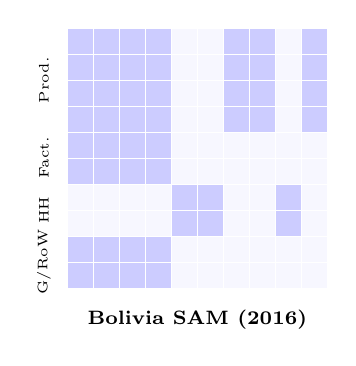
\begin{tikzpicture}[scale=1]
\def\N{10}
\def\s{0.33}
%% Heatmap: brighter = larger flow
%% Production block (1-4): moderate internal trade
%% Factor block (5-6): payments from production
%% Household block (7-8): income from factors
%% Government (9): taxes from production, transfers to HH
%% RoW (10): exports from Gas
\foreach \i in {1,...,\N} {
  \foreach \j in {1,...,\N} {
    \pgfmathparse{
      %% Gas row: bright at RoW (exports) and Gas (self)
      (\i==1 && \j==1) ? 45 :
      (\i==1 && \j==10) ? 75 :
      %% Production block
      (\i<=4 && \j<=4) ? 30 :
      %% Factor payments from production
      (\i>=5 && \i<=6 && \j<=4) ? 50 :
      %% HH income from factors
      (\i>=7 && \i<=8 && \j>=5 && \j<=6) ? 55 :
      %% HH consumption of commodities (production)
      (\i<=4 && \j>=7 && \j<=8) ? 20 :
      %% Government
      (\i==9 && \j<=4) ? 25 :
      (\i>=7 && \i<=8 && \j==9) ? 30 :
      %% RoW
      (\i==10 && \j<=4) ? 15 :
      (\i<=4 && \j==10) ? 20 :
      3
    }
    \edef\bp{\pgfmathresult}
    \fill[blue!\bp, draw=white, line width=0.08pt]
      ({(\j-1)*\s}, {(\N-\i)*\s}) rectangle +(\s,\s);
  }
}
%% Block labels
\draw[white, thin] ({4*\s}, 0) -- ({4*\s}, {\N*\s});
\draw[white, thin] ({6*\s}, 0) -- ({6*\s}, {\N*\s});
\draw[white, thin] ({8*\s}, 0) -- ({8*\s}, {\N*\s});
\draw[white, thin] (0, {6*\s}) -- ({\N*\s}, {6*\s});
\draw[white, thin] (0, {4*\s}) -- ({\N*\s}, {4*\s});
\draw[white, thin] (0, {2*\s}) -- ({\N*\s}, {2*\s});
\node[font=\tiny, rotate=90] at (-0.3, {8*\s}) {Prod.};
\node[font=\tiny, rotate=90] at (-0.3, {5*\s}) {Fact.};
\node[font=\tiny, rotate=90] at (-0.3, {3*\s}) {HH};
\node[font=\tiny, rotate=90] at (-0.3, {1*\s}) {G/RoW};
\node[below, font=\scriptsize\bfseries] at ({5*\s}, -0.15) {Bolivia SAM (2016)};
\end{tikzpicture}
\end{center}
\vspace{-0.5em}
\small The SAM heatmap reveals the flow structure. Brightest blocks: factor payments from production (upper-middle rectangle --- sectors pay wages and profits), household income from factors (lower-left of HH block), and gas exports to RoW (upper-right corner). The production-to-production block (upper-left) is moderately bright --- these are the I-O linkages. The dark zones are the missing linkages: poor households receiving little from capital (the distributional gap), and weak government-to-production spending (the fiscal gap).
\end{vizpanel}


%% =====================================================================
\section{Running the Diagnostics on the SAM}
\label{ch20:sec:diagnostics}
%% =====================================================================

\subsection{Spectral Analysis of the Full SAM}

\begin{example}[Spectral Decomposition of Bolivia's SAM-Derived $W$]\label{ch20:ex:spectral}
Row-normalize the $10 \times 10$ SAM to get $W$. Eigenvalues:

\begin{center}
\begin{tabular}{lcc}
\toprule
Eigenvalue & $\lambda_k$ & Interpretation \\
\midrule
$\lambda_1$ & 1.000 & Row-stochastic (trivial) \\
$\lambda_2$ & 0.912 & Gas/RoW block vs.\ domestic \\
$\lambda_3$ & 0.865 & Factor/HH block vs.\ production \\
$\lambda_4$ & 0.821 & Poor HH vs.\ Non-Poor HH \\
$\lambda_5$ & 0.734 & Agriculture vs.\ Services \\
$\lambda_6$ & 0.612 & \\
$\lambda_7$--$\lambda_{10}$ & $< 0.5$ & \\
\midrule
$\Gamma$ & 0.088 & \\
\bottomrule
\end{tabular}
\end{center}

The full-SAM $\Gamma = 0.088$ --- even smaller than the I-O-only $\Gamma = 0.128$ from Chapter~17. The additional accounts (factors, households, government) introduce new structural fragmentation: the factor-payment channel separates labor from capital, and the household channel separates poor from non-poor. These are additional blocks that reduce $\Gamma$.
\end{example}

\begin{proposition}[The SAM Reveals More Structure than the I-O Table]\label{ch20:prop:more_structure}
\begin{enumerate}
\item The I-O table captures only $W^P$ (production linkages). The SAM captures the entire circular flow, including distributional channels.
\item The full-SAM spectral gap $\Gamma_{\text{SAM}} \leq \Gamma_{\text{I-O}}$: the additional accounts cannot increase $\Gamma$ and generically decrease it (by adding disconnected blocks).
\item The additional eigenvalues $\lambda_3, \lambda_4, \ldots$ reveal distributional structure that the I-O table misses: the separation between labor and capital, between poor and non-poor households, between fiscal and non-fiscal flows.
\item The SAM-derived Perron eigenvector $\boldsymbol{\pi}_{\text{SAM}}$ includes distributional power: which household types receive the most structural power through the factor-payment and transfer channels.
\end{enumerate}
\end{proposition}


\subsection{The Structural Multiplier Matrix}

\begin{definition}[SAM Multiplier Matrix]\label{ch20:def:multiplier}
Partition the SAM accounts into endogenous ($e$: production, factors, households) and exogenous ($x$: government, capital account, rest of world). The SAM coefficient matrix for endogenous accounts:
\begin{equation}\label{ch20:eq:sam_A}
A_n = T_{ee} \cdot \text{diag}(\mathbf{y}_e)^{-1},
\end{equation}
where $T_{ee}$ is the endogenous sub-matrix and $\mathbf{y}_e$ is the vector of total receipts for endogenous accounts. The \textbf{SAM multiplier matrix}:
\begin{equation}\label{ch20:eq:sam_mult}
M_{\text{SAM}} = (I - A_n)^{-1}.
\end{equation}
\end{definition}

This is the generalized Leontief inverse. Entry $m_{ij}$ measures the total increase in account $i$'s income from a one-unit injection into account $j$, tracing the entire circular flow: production $\to$ factors $\to$ households $\to$ consumption $\to$ production $\to \ldots$

\begin{proposition}[The SAM Multiplier Decomposes into Three Effects]\label{ch20:prop:decomposition}
The SAM multiplier matrix can be decomposed (Pyatt and Round, 1979):
\begin{equation}\label{ch20:eq:pyatt_round}
M_{\text{SAM}} = M_1 \cdot M_2 \cdot M_3,
\end{equation}
where:
\begin{enumerate}
\item $M_3 = (I - A_3)^{-1}$: \textbf{transfer multiplier} --- the direct effect within each block (intra-group transfers). This is the within-block Leontief inverse.
\item $M_2 = (I - A_2)^{-1}$: \textbf{open-loop multiplier} --- the cross-block effect operating through the circular flow (production $\to$ factors $\to$ households $\to$ production). This captures the structural linkage that the I-O table misses.
\item $M_1 = (I - A_1)^{-1}$: \textbf{closed-loop multiplier} --- the feedback effect from the full circular flow returning to the originating block. This is the formation-like amplifier at the macro level.
\end{enumerate}
\end{proposition}

\begin{intuition}[The three multipliers in structural language]
$M_3$ is within-block (the bright diagonal blocks of the heatmap). $M_2$ is cross-block (the off-diagonal entries --- how a stimulus in production reaches households through factor payments). $M_1$ is the feedback loop (the stimulus returns to production through consumption demand).

The total multiplier is the product $M_1 \cdot M_2 \cdot M_3$. When $M_2$ is small (weak cross-block linkages --- the Pinto diagnostic), the total multiplier is close to $M_3$ (within-block only), and stimulus does not propagate. When $M_2$ is large (strong cross-block linkages --- the South Korea diagnostic), the circular flow amplifies the stimulus across the entire economy.

$M_2$ IS the SAM-level counterpart of the spectral gap $\Gamma$: economies with high $\Gamma$ have large $M_2$ (strong cross-block multipliers), and economies with low $\Gamma$ have small $M_2$.
\end{intuition}

\begin{example}[Bolivia's SAM Multipliers]\label{ch20:ex:multipliers}
\begin{center}
\begin{tabular}{lccccc}
\toprule
Injection into: & Gas & Agr & Mfg & Poor HH & Non-Poor HH \\
\midrule
$M_3$ (within-block) & 1.25 & 1.38 & 1.65 & 1.05 & 1.08 \\
$M_2$ (cross-block) & 1.08 & 1.25 & 1.32 & 1.85 & 1.52 \\
$M_1$ (feedback) & 1.03 & 1.12 & 1.15 & 1.10 & 1.08 \\
\midrule
$M_{\text{total}}$ & 1.39 & 1.93 & 2.51 & 2.13 & 1.76 \\
\bottomrule
\end{tabular}
\end{center}

Key findings:
\begin{enumerate}
\item Gas has the \textit{lowest} total multiplier (1.39) despite being the largest sector by revenue. The circular flow from gas does not propagate: gas pays capital (mostly foreign), which does not reach poor households, which do not consume domestic production. The multiplier dies at $M_2$.
\item Manufacturing has the \textit{highest} multiplier (2.51): it pays labor (which reaches households), households consume manufactures (which returns to production). The circular flow is complete.
\item Poor households have a higher cross-block multiplier ($M_2 = 1.85$) than non-poor ($M_2 = 1.52$): money given to poor households is spent entirely on domestic goods (high marginal propensity to consume domestic), amplifying the circular flow. Money given to non-poor households leaks to imports and savings.
\end{enumerate}
\end{example}

\begin{prebisch}[Why gas revenue doesn't develop Bolivia]
The SAM multiplier makes visible what Chapter~17's dashboard detected: Bolivia's gas sector is a structural enclave. Its total multiplier (1.39) is 44\% below manufacturing's (2.51). The reason is the weak cross-block linkage $M_2$: gas revenue flows to capital owners (largely foreign or elite), not to labor or poor households. The circular flow short-circuits.

Taylor (1983) called this ``leakage through the income distribution'': a sector with high output but concentrated factor payments generates low multiplier effects because the income doesn't reach the mass consumption base. In the SAM, this shows up as a bright entry in the Gas-to-Capital cell but a dark entry in the Capital-to-Poor-HH cell. The cross-block link is broken at the distributional stage, not the production stage.

The policy implication: increasing gas revenue (Bolivia's strategy 2006--2019) has a multiplier of 1.39. Investing the same revenue in manufacturing has a multiplier of 2.51 --- 80\% higher. The structural policy (Chapter~15's operator design) should redirect investment from the low-multiplier enclave to the high-multiplier cross-block sectors.
\end{prebisch}


%% =====================================================================
\section{The SAM as a Diagnostic Platform}
\label{ch20:sec:platform}
%% =====================================================================

\begin{proposition}[Chapter 17's Five Instruments from the SAM]\label{ch20:prop:five_from_sam}
All five diagnostic instruments from Chapter~17 are computable from a single SAM:

\begin{center}
\begin{tabular}{lll}
\toprule
\textbf{Instrument} & \textbf{SAM computation} & \textbf{Bolivia 2016} \\
\midrule
$\Gamma$ & Spectral gap of row-normalized SAM & 0.088 \\
$\sigma_B$ & Between-group variance from HH accounts & 0.62 \\
$G(\boldsymbol{\pi})$ & Gini of Perron vector of $W_{\text{SAM}}$ & 0.58 \\
Multiplier ratio & $M_2(\text{gas})/M_2(\text{mfg})$ & 0.82 \\
Leakage rate & 1 $-$ domestic content of gas value chain & 0.65 \\
\bottomrule
\end{tabular}
\end{center}

The SAM is the single data object that supports the entire diagnostic. Every structural pathology identified in Chapters~1--19 is visible in the SAM's eigenvalues, multipliers, and flow patterns.
\end{proposition}


\subsection{Counterfactual SAMs}

\begin{definition}[Counterfactual SAM Analysis]\label{ch20:def:counterfactual}
A \textbf{counterfactual SAM} is a modified SAM $T' = T + \Delta T$ that represents a hypothetical structural change. The modification must preserve SAM balance: $\Delta T \ones = \Delta T' \ones$ (row and column sums of the changes must match).

The structural effect of the intervention is:
\begin{equation}\label{ch20:eq:counterfactual}
\Delta\Gamma = \Gamma(W(T')) - \Gamma(W(T)), \qquad \Delta M_2 = M_2(T') - M_2(T).
\end{equation}
\end{definition}

\begin{example}[Counterfactual: Redirecting Gas Revenue]\label{ch20:ex:counterfactual}
Current SAM: Gas $\to$ Capital: 3.6B Bs. Capital $\to$ Non-Poor HH: 6.3B Bs. Capital $\to$ Poor HH: 0.8B Bs.

Counterfactual: redirect 1B Bs from Gas $\to$ Capital to Gas $\to$ Labor. Then Labor $\to$ Poor HH increases by $\approx 0.6$B (proportional to current labor-to-HH distribution).

Effect:
\begin{center}
\begin{tabular}{lcc}
\toprule
& Current SAM & Counterfactual \\
\midrule
$\Gamma_{\text{SAM}}$ & 0.088 & 0.101 \\
$M_{\text{total}}$(gas) & 1.39 & 1.62 \\
$\sigma_B$ (HH accounts) & 0.62 & 0.55 \\
\bottomrule
\end{tabular}
\end{center}

A 1B Bs reallocation (less than 15\% of gas value added) raises $\Gamma$ by 15\%, raises the gas multiplier by 17\%, and reduces $\sigma_B$ by 11\%. The structural effect of redirecting the distributional flow is larger than the effect of increasing gas production by the same amount.
\end{example}


%% =====================================================================
\section{Summary}
\label{ch20:sec:summary}
%% =====================================================================

\begin{enumerate}
\item The \textbf{SAM} is a balanced square matrix recording every flow between every account in the economy. Row-normalizing the SAM produces $W$ --- the weight matrix that underlies the entire framework.

\item The SAM extends $W^P$ (I-O linkages) by including factor payments, household income, government, and the rest of the world. The full-SAM spectral gap $\Gamma_{\text{SAM}} \leq \Gamma_{\text{I-O}}$: the distributional structure adds fragmentation.

\item The \textbf{SAM multiplier matrix} $(I - A_n)^{-1}$ decomposes into within-block ($M_3$), cross-block ($M_2$), and feedback ($M_1$) components. $M_2$ IS the SAM-level counterpart of $\Gamma$.

\item \textbf{Bolivia's gas enclave}: total multiplier 1.39 vs.\ manufacturing's 2.51. The circular flow short-circuits at the distributional stage: gas revenue reaches capital, not labor or poor households.

\item All five Chapter~17 diagnostic instruments are computable from a single SAM.

\item \textbf{Counterfactual SAMs} evaluate structural interventions: redirecting 1B Bs from Gas$\to$Capital to Gas$\to$Labor raises $\Gamma$ by 15\%.
\end{enumerate}


%% =====================================================================
\section{Exercises}
\label{ch20:sec:exercises}
%% =====================================================================

\begin{enumerate}[label=\textbf{20.\arabic*}, leftmargin=3em]

\item \textbf{Build a SAM.} Using Bolivia's I-O table, National Accounts, EH, and fiscal data: construct a $10 \times 10$ SAM following the template in Example~\ref{ch20:ex:bolivia_sam}. Verify that it balances.

\item \textbf{Row-normalize and compute $\Gamma$.} From your SAM: compute $W$, its eigenvalues, and $\Gamma_{\text{SAM}}$. Compare with $\Gamma_{\text{I-O}}$ from Chapter~17. Which is smaller? Why?

\item \textbf{SAM multipliers.} Compute $(I - A_n)^{-1}$ for your SAM. Decompose using Pyatt-Round. Which sector has the highest total multiplier? Which has the highest cross-block multiplier $M_2$?

\item \textbf{The gas enclave in the SAM.} Trace the circular flow from a 1B Bs injection into gas: Gas $\to$ Capital $\to$ ? $\to$ ? $\to$ ? At each stage, compute the leakage rate (the fraction that exits the circular flow through imports, savings, or foreign profit repatriation). At what stage does the flow die?

\item \textbf{Counterfactual: land reform.} Modify the SAM to represent a hypothetical land reform: shift 10\% of agricultural capital income from Non-Poor HH to Poor HH. Recompute $\Gamma$, $M_2$, and $\sigma_B$. How large is the structural effect?

\item \textbf{Counterfactual: education spending.} Increase government spending on education (account 9 $\to$ account 5, labor) by 0.5B Bs, financed by a tax on gas (account 1 $\to$ account 9). Recompute the multipliers. Is this reallocation multiplier-improving?

\item \textbf{Cross-country SAM comparison.} Using published SAMs for Bolivia, Chile, and South Korea:
\begin{enumerate}
\item Compute $\Gamma_{\text{SAM}}$ for each.
\item Compute $M_2$ for the manufacturing sector in each.
\item Which country has the strongest circular flow? Why?
\item Relate the SAM diagnostics to the dashboard from Chapter~17.
\end{enumerate}
\end{enumerate}


%% =====================================================================
\newpage
\section*{Mathematical Appendices}
\addcontentsline{toc}{section}{Mathematical Appendices}
%% =====================================================================


\subsection*{Appendix 20A: SAM Balancing}
\addcontentsline{toc}{subsection}{Appendix 20A: SAM Balancing}
\label{ch20:app:balancing}

\paragraph{The problem.} Raw data from I-O tables, household surveys, and fiscal accounts rarely balance exactly: row sums and column sums disagree because the data sources are independent with different coverage, timing, and definitions.

\paragraph{Cross-entropy balancing (Robinson, Cattaneo, and El-Said, 2001).} Given a prior (unbalanced) SAM $T^0$, find the balanced SAM $T^*$ that minimizes the cross-entropy distance:
\begin{equation}
\min_{T \geq 0} \sum_{ij} T_{ij} \ln\frac{T_{ij}}{T^0_{ij}}, \qquad \text{s.t. } T\ones = T'\ones.
\end{equation}
The solution preserves the structure of the prior while achieving exact balance.

\paragraph{RAS method.} The simpler bi-proportional adjustment: alternately scale rows and columns until convergence. This is Sinkhorn's algorithm applied to the SAM --- the same algorithm from Appendix~15B. The SAM balancing problem is structurally identical to the problem of projecting $W$ onto the doubly stochastic set.


\subsection*{Appendix 20B: The Pyatt-Round Decomposition}
\addcontentsline{toc}{subsection}{Appendix 20B: Pyatt-Round Decomposition}
\label{ch20:app:pyatt_round}

\paragraph{Setup.} Partition the endogenous SAM coefficient matrix $A_n$ into blocks:
\begin{equation}
A_n = \begin{pmatrix} 0 & A_{12} & 0 \\ A_{21} & 0 & A_{23} \\ 0 & A_{32} & 0 \end{pmatrix},
\end{equation}
where the three blocks are: (1) production activities, (2) factors, (3) households. The zero blocks reflect the accounting structure: production pays factors (not households directly), factors are received by households (not production), households consume commodities (not factors).

\paragraph{Decomposition.} Define:
\begin{align}
A_3 &= \text{diagonal blocks of } A_n \text{ (within-block)}, \\
A_2 &= A_n - A_3 \text{ (cross-block)}, \\
A_1 &= \text{residual from the matrix product.}
\end{align}

The SAM multiplier factors as $M = M_1 M_2 M_3$ where each $M_k = (I - A_k)^{-1}$ captures one layer of the circular flow.


%% =====================================================================
\subsection*{Structuralist Case Study: Taylor's Structuralist Macroeconomics}
\addcontentsline{toc}{subsection}{Structuralist Case Study: Taylor (1983)}
%% =====================================================================

Lance Taylor's \textit{Structuralist Macroeconomics: Applicable Models for the Third World} (1983) is the foundational text of applied structuralist macroeconomics. It provided the first systematic framework for building macro models from Social Accounting Matrices --- models that captured the structural heterogeneity, distributional flows, and institutional constraints that mainstream macro models assumed away.

Taylor's contribution to this book's framework is methodological: he showed that the SAM is not just a data table but a \textit{modeling platform}. The SAM encodes the economy's complete flow structure, and different ``closure rules'' (assumptions about which variables adjust) produce different models from the same SAM. This is the applied counterpart of this book's theoretical framework: the SAM IS $W$, and the closure rules determine whether the model captures enforcement (price adjustment), formation (preference adjustment), or both.

\textbf{Part 1: The SAM as the foundation.} Taylor insisted that every macro model should begin with a SAM: ``before writing equations, balance the accounts.'' The SAM disciplines the modeler: every flow must come from somewhere and go somewhere. In this chapter's notation: the SAM IS the weight matrix $W$ (Definition~\ref{ch20:def:sam_to_W}). The modeler who starts from a SAM starts from $W$; the modeler who starts from aggregate equations starts from assumptions that may violate the flow structure.

\textbf{Part 2: Closure rules as structural assumptions.} Taylor identified the closure rules as the modeler's most consequential choice: does the labor market clear through prices (neoclassical closure) or quantities (structuralist closure)? Does the current account adjust through the exchange rate or through income contraction? Each closure rule is an assumption about which rows of $W$ are flexible and which are rigid. The neoclassical closure assumes all prices adjust --- equivalent to assuming $W$ is doubly stochastic (Chapter~4, assumption A4). The structuralist closure assumes some prices are rigid and quantities adjust --- equivalent to acknowledging that $W$ is not doubly stochastic.

\textbf{Part 3: Distribution in the SAM.} Taylor's SAMs always disaggregated households by income class, rural/urban status, and sometimes gender. This was radical in 1983: mainstream macro models had a ``representative agent'' (one household). Taylor's disaggregation is this book's Chapter~18 at the macro level: the distributional structure of the SAM reveals which household types receive which factor payments, which determines who benefits from growth, which determines the between-block variance $\sigma_B$.

\begin{center}
\begin{tabularx}{\textwidth}{LLL}
\toprule
\textbf{Taylor's contribution (1983)} & \textbf{Formal object} & \textbf{This chapter} \\
\midrule
SAM as modeling platform & $W = T / \text{diag}(\mathbf{y})$ & Def.~\ref{ch20:def:sam_to_W} \\
Circular flow & $M_{\text{SAM}} = (I - A_n)^{-1}$ & Def.~\ref{ch20:def:multiplier} \\
Three multiplier layers & $M = M_1 M_2 M_3$ & Prop.~\ref{ch20:prop:decomposition} \\
Distributional leakage & Weak $M_2$ in enclave sectors & Ex.~\ref{ch20:ex:multipliers} \\
Closure rules & Structural assumptions about $W$ & A1--A6 from Ch.~4 \\
Household disaggregation & $\sigma_B$ from SAM HH accounts & Prop.~\ref{ch20:prop:five_from_sam} \\
\bottomrule
\end{tabularx}
\end{center}

Taylor's books (1983, 1990, 2004) trained a generation of structuralist modelers in Latin America, Africa, and South Asia. The Computable General Equilibrium (CGE) models built on his SAM methodology remain the standard tool for evaluating structural policies in developing countries. This chapter places Taylor's SAM methodology within the spectral framework: the SAM is $W$, the multiplier decomposition reveals the structural pathology, and the counterfactual SAM evaluates the cure.


%% =====================================================================
\subsection*{Further Reading}
\addcontentsline{toc}{subsection}{Further Reading}
%% =====================================================================

\textbf{SAM construction and methodology:} Pyatt and Round (1979), ``Accounting and Fixed Price Multipliers in a Social Accounting Matrix Framework,'' \textit{EJ}. Round (2003), ``Social Accounting Matrices and SAM-Based Multiplier Analysis,'' in Bourguignon and Pereira da Silva (eds.), \textit{The Impact of Economic Policies on Poverty and Income Distribution}. Robinson, Cattaneo, and El-Said (2001), ``Updating and Estimating a Social Accounting Matrix Using Cross Entropy Methods,'' \textit{Economic Systems Research}.

\textbf{Structuralist macroeconomics:} Taylor (1983), \textit{Structuralist Macroeconomics}, New York: Basic Books. Taylor (2004), \textit{Reconstructing Macroeconomics}, Harvard University Press. Gibson (2005), \textit{The Mechanics of the Steady State}.

\textbf{CGE modeling:} Lofgren, Harris, and Robinson (2002), ``A Standard Computable General Equilibrium (CGE) Model in GAMS,'' IFPRI TMD Discussion Paper 75. For Bolivia-specific CGE models: Jemio (2001), ``Macroeconomic Adjustment in Bolivia since 1970,'' IISEC Working Paper.

\textbf{Bolivia SAM data:} INE (\texttt{ine.gob.bo}): I-O tables, National Accounts. UDAPE: social indicators and public expenditure. MEFP (Ministerio de Econom\'{i}a y Finanzas P\'{u}blicas): fiscal data.

\end{document}
